% Options for packages loaded elsewhere
\PassOptionsToPackage{unicode}{hyperref}
\PassOptionsToPackage{hyphens}{url}
%
\documentclass[
]{article}
\usepackage{lmodern}
\usepackage{amssymb,amsmath}
\usepackage{ifxetex,ifluatex}
\ifnum 0\ifxetex 1\fi\ifluatex 1\fi=0 % if pdftex
  \usepackage[T1]{fontenc}
  \usepackage[utf8]{inputenc}
  \usepackage{textcomp} % provide euro and other symbols
\else % if luatex or xetex
  \usepackage{unicode-math}
  \defaultfontfeatures{Scale=MatchLowercase}
  \defaultfontfeatures[\rmfamily]{Ligatures=TeX,Scale=1}
\fi
% Use upquote if available, for straight quotes in verbatim environments
\IfFileExists{upquote.sty}{\usepackage{upquote}}{}
\IfFileExists{microtype.sty}{% use microtype if available
  \usepackage[]{microtype}
  \UseMicrotypeSet[protrusion]{basicmath} % disable protrusion for tt fonts
}{}
\makeatletter
\@ifundefined{KOMAClassName}{% if non-KOMA class
  \IfFileExists{parskip.sty}{%
    \usepackage{parskip}
  }{% else
    \setlength{\parindent}{0pt}
    \setlength{\parskip}{6pt plus 2pt minus 1pt}}
}{% if KOMA class
  \KOMAoptions{parskip=half}}
\makeatother
\usepackage{xcolor}
\IfFileExists{xurl.sty}{\usepackage{xurl}}{} % add URL line breaks if available
\IfFileExists{bookmark.sty}{\usepackage{bookmark}}{\usepackage{hyperref}}
\hypersetup{
  pdftitle={Week 2 Tutorial},
  pdfauthor={Maria Prokofieva},
  hidelinks,
  pdfcreator={LaTeX via pandoc}}
\urlstyle{same} % disable monospaced font for URLs
\usepackage[margin=1in]{geometry}
\usepackage{color}
\usepackage{fancyvrb}
\newcommand{\VerbBar}{|}
\newcommand{\VERB}{\Verb[commandchars=\\\{\}]}
\DefineVerbatimEnvironment{Highlighting}{Verbatim}{commandchars=\\\{\}}
% Add ',fontsize=\small' for more characters per line
\usepackage{framed}
\definecolor{shadecolor}{RGB}{248,248,248}
\newenvironment{Shaded}{\begin{snugshade}}{\end{snugshade}}
\newcommand{\AlertTok}[1]{\textcolor[rgb]{0.94,0.16,0.16}{#1}}
\newcommand{\AnnotationTok}[1]{\textcolor[rgb]{0.56,0.35,0.01}{\textbf{\textit{#1}}}}
\newcommand{\AttributeTok}[1]{\textcolor[rgb]{0.77,0.63,0.00}{#1}}
\newcommand{\BaseNTok}[1]{\textcolor[rgb]{0.00,0.00,0.81}{#1}}
\newcommand{\BuiltInTok}[1]{#1}
\newcommand{\CharTok}[1]{\textcolor[rgb]{0.31,0.60,0.02}{#1}}
\newcommand{\CommentTok}[1]{\textcolor[rgb]{0.56,0.35,0.01}{\textit{#1}}}
\newcommand{\CommentVarTok}[1]{\textcolor[rgb]{0.56,0.35,0.01}{\textbf{\textit{#1}}}}
\newcommand{\ConstantTok}[1]{\textcolor[rgb]{0.00,0.00,0.00}{#1}}
\newcommand{\ControlFlowTok}[1]{\textcolor[rgb]{0.13,0.29,0.53}{\textbf{#1}}}
\newcommand{\DataTypeTok}[1]{\textcolor[rgb]{0.13,0.29,0.53}{#1}}
\newcommand{\DecValTok}[1]{\textcolor[rgb]{0.00,0.00,0.81}{#1}}
\newcommand{\DocumentationTok}[1]{\textcolor[rgb]{0.56,0.35,0.01}{\textbf{\textit{#1}}}}
\newcommand{\ErrorTok}[1]{\textcolor[rgb]{0.64,0.00,0.00}{\textbf{#1}}}
\newcommand{\ExtensionTok}[1]{#1}
\newcommand{\FloatTok}[1]{\textcolor[rgb]{0.00,0.00,0.81}{#1}}
\newcommand{\FunctionTok}[1]{\textcolor[rgb]{0.00,0.00,0.00}{#1}}
\newcommand{\ImportTok}[1]{#1}
\newcommand{\InformationTok}[1]{\textcolor[rgb]{0.56,0.35,0.01}{\textbf{\textit{#1}}}}
\newcommand{\KeywordTok}[1]{\textcolor[rgb]{0.13,0.29,0.53}{\textbf{#1}}}
\newcommand{\NormalTok}[1]{#1}
\newcommand{\OperatorTok}[1]{\textcolor[rgb]{0.81,0.36,0.00}{\textbf{#1}}}
\newcommand{\OtherTok}[1]{\textcolor[rgb]{0.56,0.35,0.01}{#1}}
\newcommand{\PreprocessorTok}[1]{\textcolor[rgb]{0.56,0.35,0.01}{\textit{#1}}}
\newcommand{\RegionMarkerTok}[1]{#1}
\newcommand{\SpecialCharTok}[1]{\textcolor[rgb]{0.00,0.00,0.00}{#1}}
\newcommand{\SpecialStringTok}[1]{\textcolor[rgb]{0.31,0.60,0.02}{#1}}
\newcommand{\StringTok}[1]{\textcolor[rgb]{0.31,0.60,0.02}{#1}}
\newcommand{\VariableTok}[1]{\textcolor[rgb]{0.00,0.00,0.00}{#1}}
\newcommand{\VerbatimStringTok}[1]{\textcolor[rgb]{0.31,0.60,0.02}{#1}}
\newcommand{\WarningTok}[1]{\textcolor[rgb]{0.56,0.35,0.01}{\textbf{\textit{#1}}}}
\usepackage{graphicx,grffile}
\makeatletter
\def\maxwidth{\ifdim\Gin@nat@width>\linewidth\linewidth\else\Gin@nat@width\fi}
\def\maxheight{\ifdim\Gin@nat@height>\textheight\textheight\else\Gin@nat@height\fi}
\makeatother
% Scale images if necessary, so that they will not overflow the page
% margins by default, and it is still possible to overwrite the defaults
% using explicit options in \includegraphics[width, height, ...]{}
\setkeys{Gin}{width=\maxwidth,height=\maxheight,keepaspectratio}
% Set default figure placement to htbp
\makeatletter
\def\fps@figure{htbp}
\makeatother
\setlength{\emergencystretch}{3em} % prevent overfull lines
\providecommand{\tightlist}{%
  \setlength{\itemsep}{0pt}\setlength{\parskip}{0pt}}
\setcounter{secnumdepth}{-\maxdimen} % remove section numbering

\title{Week 2 Tutorial}
\author{Maria Prokofieva}
\date{15/01/2020}

\begin{document}
\maketitle

\hypertarget{week-2-basics-of-data-viz}{%
\subsection{Week 2: Basics of data
viz}\label{week-2-basics-of-data-viz}}

This week we are getting into data viz with R. We already started
working with RMarkdown - which is ``file format'' to present your data
insights and communicate them to stakeholders

A screencast of the tutorial is available
\href{https://www.youtube.com/channel/UCTpTqzAm8DCANz7ifhRI-sA?disable_polymer=true}{here}:

\hypertarget{things-to-cover}{%
\subsubsection{Things to cover:}\label{things-to-cover}}

\begin{enumerate}
\def\labelenumi{\arabic{enumi}.}
\tightlist
\item
  Basics of RMarkdown
\item
  \texttt{ggplot2} library: install and start using
\item
  Working with basic data viz
\end{enumerate}

Remember: \textbf{This is not a programming unit! We focus on data and
working with data}

\hypertarget{what-i-need-to-learn}{%
\subsubsection{What I need to learn:}\label{what-i-need-to-learn}}

\begin{itemize}
\tightlist
\item
  work with \texttt{RMarkdown} documents with dataviz
\item
  install and load \texttt{ggplot2} library
\item
  work with layers in the grammar of gpaphics in \texttt{ggplot2}
\item
  create basics dataviz ``shapes'': e.g.~histograms, line charts, etc.
  in \texttt{ggplot2}
\item
  use colour in your data viz in \texttt{ggplot2}
\item
  use themes in \texttt{ggplot2}
\item
  use legends, labels and axes names
\item
  use faceting and present multiple data insights on one data viz
\end{itemize}

\hypertarget{resources}{%
\subsubsection{Resources}\label{resources}}

ggplot2: Elegant Graphics for Data Analysis
\url{https://ggplot2-book.org/}

RMarkdown: \url{https://rmarkdown.rstudio.com/lesson-1.html}

Markdown - syntax:
\url{https://github.com/adam-p/markdown-here/wiki/Markdown-Cheatsheet}

\begin{center}\rule{0.5\linewidth}{0.5pt}\end{center}

\hypertarget{using-data-viz-in-rmarkdown}{%
\subsubsection{\texorpdfstring{Using data viz in
\texttt{RMarkdown}}{Using data viz in RMarkdown}}\label{using-data-viz-in-rmarkdown}}

This tutorial we are going to have a closer look at \texttt{RMarkdown}
and put out data viz there

\hypertarget{task}{%
\subsubsection{Task}\label{task}}

\begin{itemize}
\tightlist
\item
  create an RMarkdown document and select \texttt{html} as output - this
  tells R to create an \texttt{html\ document} when you knit it (you can
  later swap it to \texttt{Word\ document})
\end{itemize}

\hypertarget{working-with-meta-data-section}{%
\paragraph{Working with meta-data
section}\label{working-with-meta-data-section}}

\begin{itemize}
\tightlist
\item
  Look at the structure of the document and syntax used. Locate the
  following:
\end{itemize}

⋅⋅* meta-data section ⋅⋅* R code chuncks ⋅⋅* text

\begin{itemize}
\item
  Locate the section in the meta-data section that specifies the output
\item
  Locate the section in the meta-data that specifies \texttt{title},
  \texttt{author} and \texttt{title}. Change these sections to include
  your details. Use \texttt{Knit} button to regenerate the document.
  Review your changes.
\end{itemize}

\hypertarget{working-with-r-code}{%
\subparagraph{Working with R code}\label{working-with-r-code}}

\begin{itemize}
\tightlist
\item
  Locate the section that specifies \texttt{R\ code}. Review the manual
  and locate inline code and code chunks.
\end{itemize}

\hypertarget{text-editing}{%
\paragraph{Text editing}\label{text-editing}}

\begin{itemize}
\item
  Locate the line that includes ``R Markdown'' heading and change it to
  ``R Markdown description''. Use \texttt{Knit} button to regenerate the
  document. Review your changes.
\item
  Move to the paragraph and edit it. Regenerate the document in the same
  way and review your changes.
\end{itemize}

\hypertarget{markdown-vs-rmarkdown}{%
\subparagraph{Markdown vs RMarkdown}\label{markdown-vs-rmarkdown}}

Working with text section of your file, you are using ``plain''
\texttt{Markdown}, but including \texttt{R\ Chunks} makes it
\texttt{RMarkdown}

\texttt{Markdown} is very simple. Review the following to get
\href{https://github.com/adam-p/markdown-here/wiki/Markdown-Cheatsheet}{basics}

Review the structure of the document and \textbf{Markdown} guide and
answer the following questions:

\begin{itemize}
\item
  How to create different level headings?
\item
  How to include lists?
\item
  How to include links?
\item
  How to include images? Upload any image to your RStudio.cloud folder
  and include it in the text.
\end{itemize}

\begin{center}\rule{0.5\linewidth}{0.5pt}\end{center}

\hypertarget{working-with-ggplot2}{%
\subsubsection{\texorpdfstring{Working with
\texttt{ggplot2}}{Working with ggplot2}}\label{working-with-ggplot2}}

We will be changing the document further to include basics dataviz.

Remember that to use a library it needs to be

\begin{enumerate}
\def\labelenumi{\arabic{enumi}.}
\item
  Installed on your computer using \texttt{install.packages("ggplot2")}
  - you do it only \textbf{ONCE}
\item
  Load the library in every file you use it (do not forget to run it!)
  using \texttt{library(ggplot2)}
\end{enumerate}

\begin{Shaded}
\begin{Highlighting}[]
\CommentTok{#install.packages("ggplot2") $ this is commented out so it does not install EVERY TIME you knit your file. }

\KeywordTok{library}\NormalTok{(ggplot2)}
\KeywordTok{library}\NormalTok{(tidyverse) }\CommentTok{#ggplot2 is part of tidyverse, so you can load only one.}
\CommentTok{# make sure that you install tidyverse first using install.packages("tidyverse)}
\end{Highlighting}
\end{Shaded}

We will be working with one of the default datasets, \texttt{mpg}

\begin{Shaded}
\begin{Highlighting}[]
\NormalTok{dataset<-mpg}
\KeywordTok{head}\NormalTok{(dataset, }\DataTypeTok{format =} \StringTok{"html"}\NormalTok{)}
\CommentTok{# # A tibble: 6 x 11}
\CommentTok{#   manufacturer model displ  year   cyl trans      drv     cty   hwy fl    class }
\CommentTok{#   <chr>        <chr> <dbl> <int> <int> <chr>      <chr> <int> <int> <chr> <chr> }
\CommentTok{# 1 audi         a4      1.8  1999     4 auto(l5)   f        18    29 p     compa~}
\CommentTok{# 2 audi         a4      1.8  1999     4 manual(m5) f        21    29 p     compa~}
\CommentTok{# 3 audi         a4      2    2008     4 manual(m6) f        20    31 p     compa~}
\CommentTok{# 4 audi         a4      2    2008     4 auto(av)   f        21    30 p     compa~}
\CommentTok{# 5 audi         a4      2.8  1999     6 auto(l5)   f        16    26 p     compa~}
\CommentTok{# 6 audi         a4      2.8  1999     6 manual(m5) f        18    26 p     compa~}

\KeywordTok{glimpse}\NormalTok{(dataset)}
\CommentTok{# Rows: 234}
\CommentTok{# Columns: 11}
\CommentTok{# $ manufacturer <chr> "audi", "audi", "audi", "audi", "audi", "audi", "audi"...}
\CommentTok{# $ model        <chr> "a4", "a4", "a4", "a4", "a4", "a4", "a4", "a4 quattro"...}
\CommentTok{# $ displ        <dbl> 1.8, 1.8, 2.0, 2.0, 2.8, 2.8, 3.1, 1.8, 1.8, 2.0, 2.0,...}
\CommentTok{# $ year         <int> 1999, 1999, 2008, 2008, 1999, 1999, 2008, 1999, 1999, ...}
\CommentTok{# $ cyl          <int> 4, 4, 4, 4, 6, 6, 6, 4, 4, 4, 4, 6, 6, 6, 6, 6, 6, 8, ...}
\CommentTok{# $ trans        <chr> "auto(l5)", "manual(m5)", "manual(m6)", "auto(av)", "a...}
\CommentTok{# $ drv          <chr> "f", "f", "f", "f", "f", "f", "f", "4", "4", "4", "4",...}
\CommentTok{# $ cty          <int> 18, 21, 20, 21, 16, 18, 18, 18, 16, 20, 19, 15, 17, 17...}
\CommentTok{# $ hwy          <int> 29, 29, 31, 30, 26, 26, 27, 26, 25, 28, 27, 25, 25, 25...}
\CommentTok{# $ fl           <chr> "p", "p", "p", "p", "p", "p", "p", "p", "p", "p", "p",...}
\CommentTok{# $ class        <chr> "compact", "compact", "compact", "compact", "compact",...}

\CommentTok{#you can also display your data in a nicer way using kable() function from knitr package}
\CommentTok{#install.packages("knitr")}
\KeywordTok{library}\NormalTok{(knitr)}

\KeywordTok{kable}\NormalTok{(dataset[}\DecValTok{1}\OperatorTok{:}\DecValTok{5}\NormalTok{,], }\DataTypeTok{format =} \StringTok{"html"}\NormalTok{, }\DataTypeTok{caption =} \StringTok{"Dataset mpg"}\NormalTok{)}
\end{Highlighting}
\end{Shaded}

Dataset mpg

manufacturer

model

displ

year

cyl

trans

drv

cty

hwy

fl

class

audi

a4

1.8

1999

4

auto(l5)

f

18

29

p

compact

audi

a4

1.8

1999

4

manual(m5)

f

21

29

p

compact

audi

a4

2.0

2008

4

manual(m6)

f

20

31

p

compact

audi

a4

2.0

2008

4

auto(av)

f

21

30

p

compact

audi

a4

2.8

1999

6

auto(l5)

f

16

26

p

compact

\textbf{Task}

\begin{enumerate}
\def\labelenumi{\arabic{enumi}.}
\tightlist
\item
  Review \texttt{Help} for \texttt{kable} function and locate
\end{enumerate}

\begin{itemize}
\item
  How to specify the dataset to display
\item
  How to specify number of rows and columns to display
\item
  How to use \texttt{row.names} and \texttt{col.names}
\item
  How to use \texttt{caption}
\item
  How to use \texttt{align}
\end{itemize}

\begin{enumerate}
\def\labelenumi{\arabic{enumi}.}
\setcounter{enumi}{1}
\tightlist
\item
  Use \texttt{Help} to locate information about \texttt{mpg}
\end{enumerate}

\hypertarget{ggplot2-components}{%
\paragraph{ggplot2 components}\label{ggplot2-components}}

Every ggplot2 plot has three key components:

\begin{itemize}
\item
  \textbf{data},
\item
  A set of \textbf{aesthetic mappings} between variables in the data and
  visual properties, and
\item
  At least \textbf{one layer} (usually \texttt{geom\_something}
  function) which describes how to render each observation.
\end{itemize}

\textbf{Tasks}:

\begin{enumerate}
\def\labelenumi{\arabic{enumi}.}
\tightlist
\item
  Look at the code below and locate all 3 components
\end{enumerate}

\begin{Shaded}
\begin{Highlighting}[]
\KeywordTok{ggplot}\NormalTok{(dataset, }\KeywordTok{aes}\NormalTok{(}\DataTypeTok{x =}\NormalTok{ displ, }\DataTypeTok{y =}\NormalTok{ hwy)) }\OperatorTok{+}\StringTok{ }
\StringTok{  }\KeywordTok{geom_point}\NormalTok{()}
\end{Highlighting}
\end{Shaded}

\begin{center}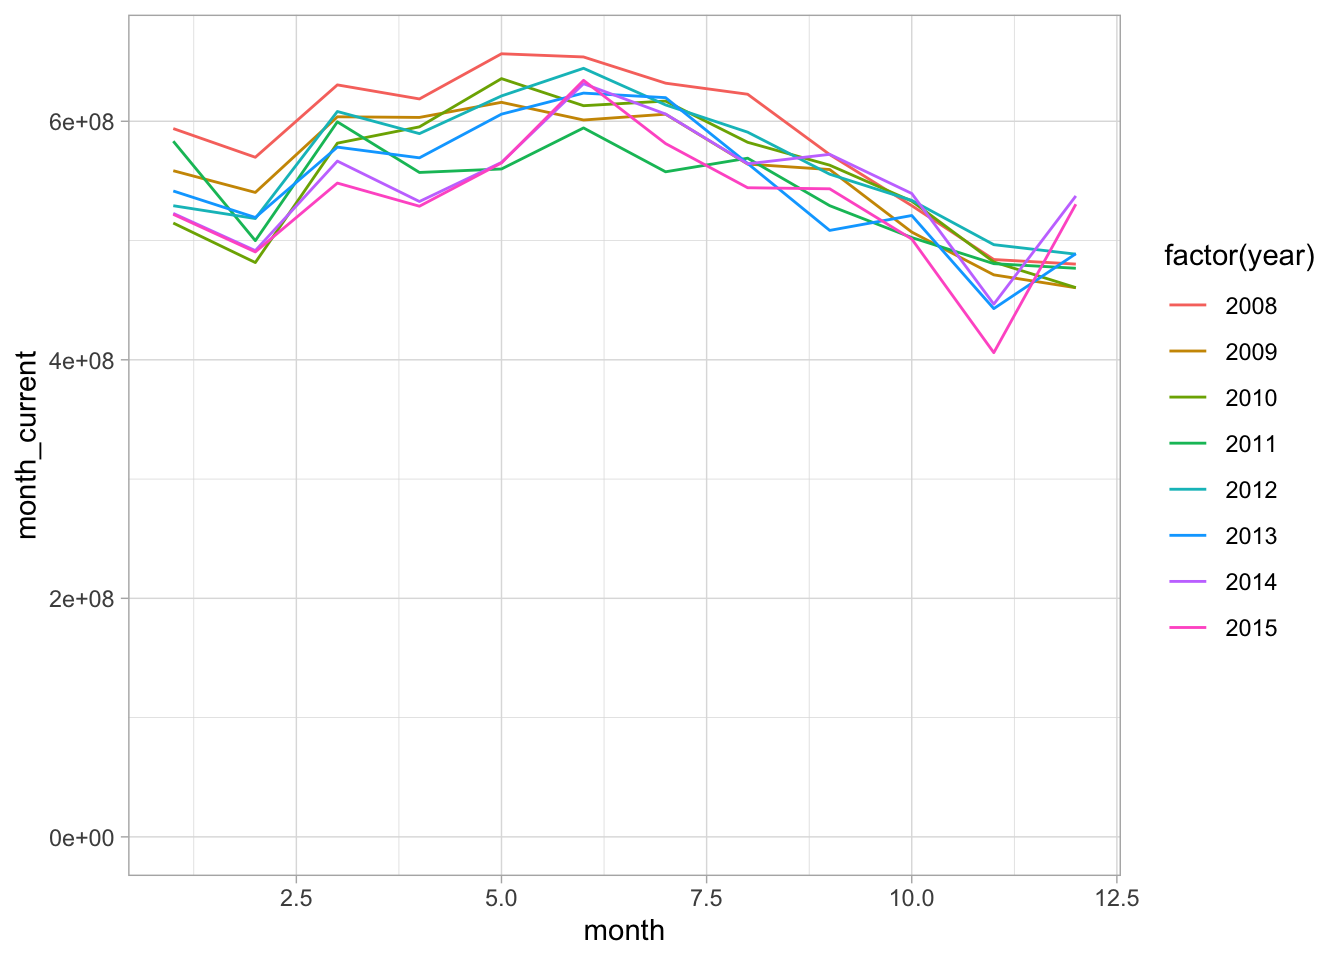
\includegraphics{week2_files/figure-latex/unnamed-chunk-4-1} \end{center}

\begin{enumerate}
\def\labelenumi{\arabic{enumi}.}
\setcounter{enumi}{1}
\tightlist
\item
  Change the code to map different variables to aesthetics:
  \texttt{model} and \texttt{manufacturer}
\end{enumerate}

Is it useful? How could you modify the data to make it more informative?

\begin{enumerate}
\def\labelenumi{\arabic{enumi}.}
\setcounter{enumi}{2}
\tightlist
\item
  Change the code to use a different \texttt{geom} -
  \texttt{geom\_count}
\end{enumerate}

Review the \texttt{ggplot2} cheatsheet in the VU Collaborate (you can
also access it via your RStudio cloud account)

\begin{enumerate}
\def\labelenumi{\arabic{enumi}.}
\setcounter{enumi}{3}
\tightlist
\item
  Review the following code to identify components, run the code by
  typing it yourself and change the code to use different mapping/geoms.
  Use ggplot2 cheatsheet to locate most suitable types of geoms.
\end{enumerate}

\begin{Shaded}
\begin{Highlighting}[]
\KeywordTok{ggplot}\NormalTok{(mpg, }\KeywordTok{aes}\NormalTok{(cty, hwy)) }\OperatorTok{+}\StringTok{ }\KeywordTok{geom_point}\NormalTok{()}
\KeywordTok{ggplot}\NormalTok{(diamonds, }\KeywordTok{aes}\NormalTok{(carat, price)) }\OperatorTok{+}\StringTok{ }\KeywordTok{geom_point}\NormalTok{()}
\KeywordTok{ggplot}\NormalTok{(economics, }\KeywordTok{aes}\NormalTok{(date, unemploy)) }\OperatorTok{+}\StringTok{ }\KeywordTok{geom_line}\NormalTok{()}
\KeywordTok{ggplot}\NormalTok{(mpg, }\KeywordTok{aes}\NormalTok{(cty)) }\OperatorTok{+}\StringTok{ }\KeywordTok{geom_histogram}\NormalTok{()}
\end{Highlighting}
\end{Shaded}

To add additional variables to a plot, we can use other aesthetics: -
colour, - shape, and - size

These work in the same way as the x and y aesthetics, and are added into
to \texttt{aes()}:

\begin{Shaded}
\begin{Highlighting}[]
\KeywordTok{aes}\NormalTok{(displ, hwy, }\DataTypeTok{colour =}\NormalTok{ class)}
\KeywordTok{aes}\NormalTok{(displ, hwy, }\DataTypeTok{shape =}\NormalTok{ drv)}
\KeywordTok{aes}\NormalTok{(displ, hwy, }\DataTypeTok{size =}\NormalTok{ cyl)}
\end{Highlighting}
\end{Shaded}

Look the following example and replace the variable that you use to map
in \texttt{colour}. Notice the type of variable that you can use:

\begin{Shaded}
\begin{Highlighting}[]
\KeywordTok{ggplot}\NormalTok{(dataset, }\KeywordTok{aes}\NormalTok{(displ, cty, }\DataTypeTok{colour =}\NormalTok{ class)) }\OperatorTok{+}\StringTok{ }
\StringTok{  }\KeywordTok{geom_point}\NormalTok{()}
\end{Highlighting}
\end{Shaded}

\begin{center}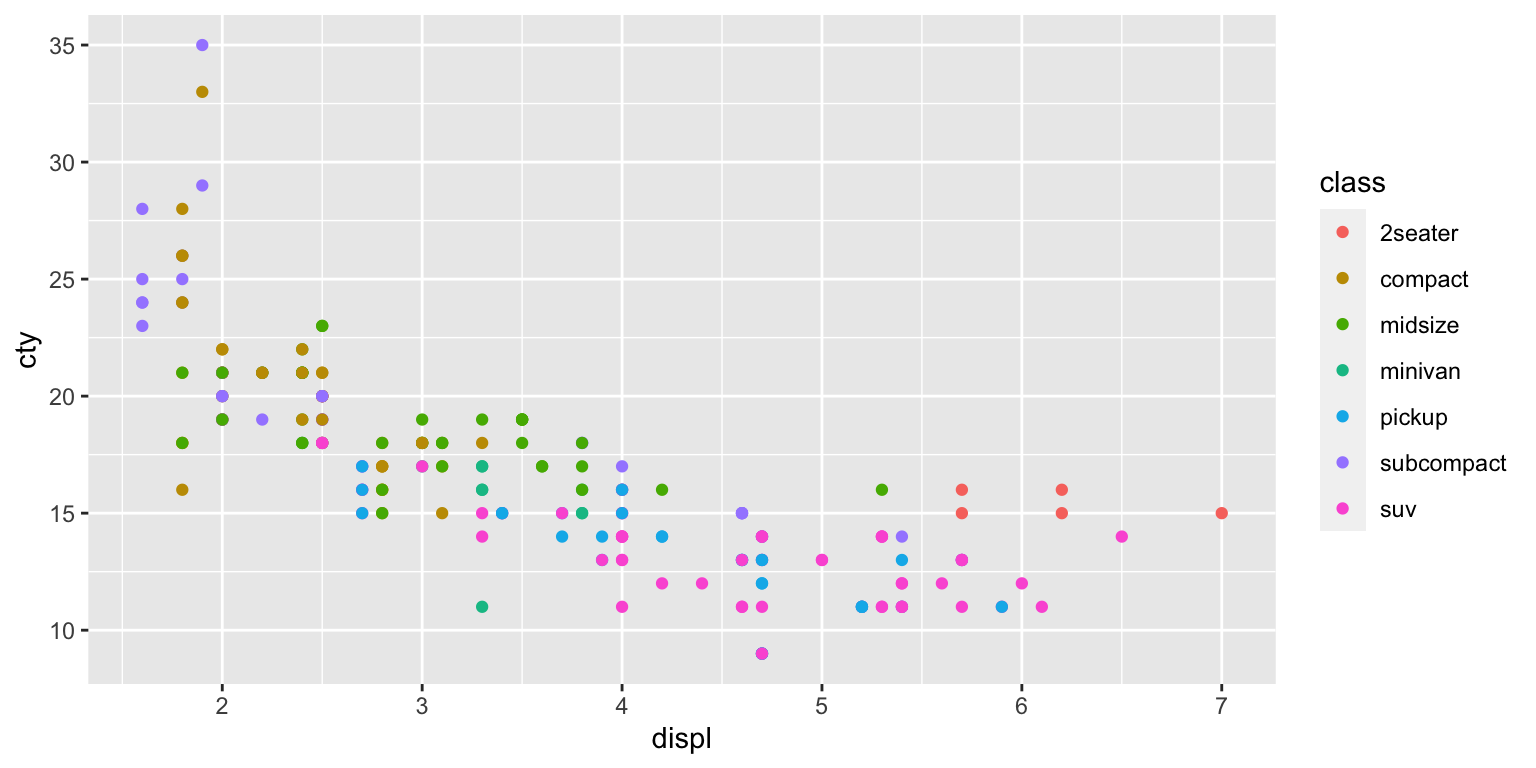
\includegraphics{week2_files/figure-latex/unnamed-chunk-7-1} \end{center}

Compare the following plots and note the component to use for colour and
the outcome:

\begin{Shaded}
\begin{Highlighting}[]
\KeywordTok{ggplot}\NormalTok{(dataset, }\KeywordTok{aes}\NormalTok{(displ, hwy)) }\OperatorTok{+}\StringTok{ }\KeywordTok{geom_point}\NormalTok{(}\KeywordTok{aes}\NormalTok{(}\DataTypeTok{colour =} \StringTok{"blue"}\NormalTok{))}
\end{Highlighting}
\end{Shaded}

\begin{center}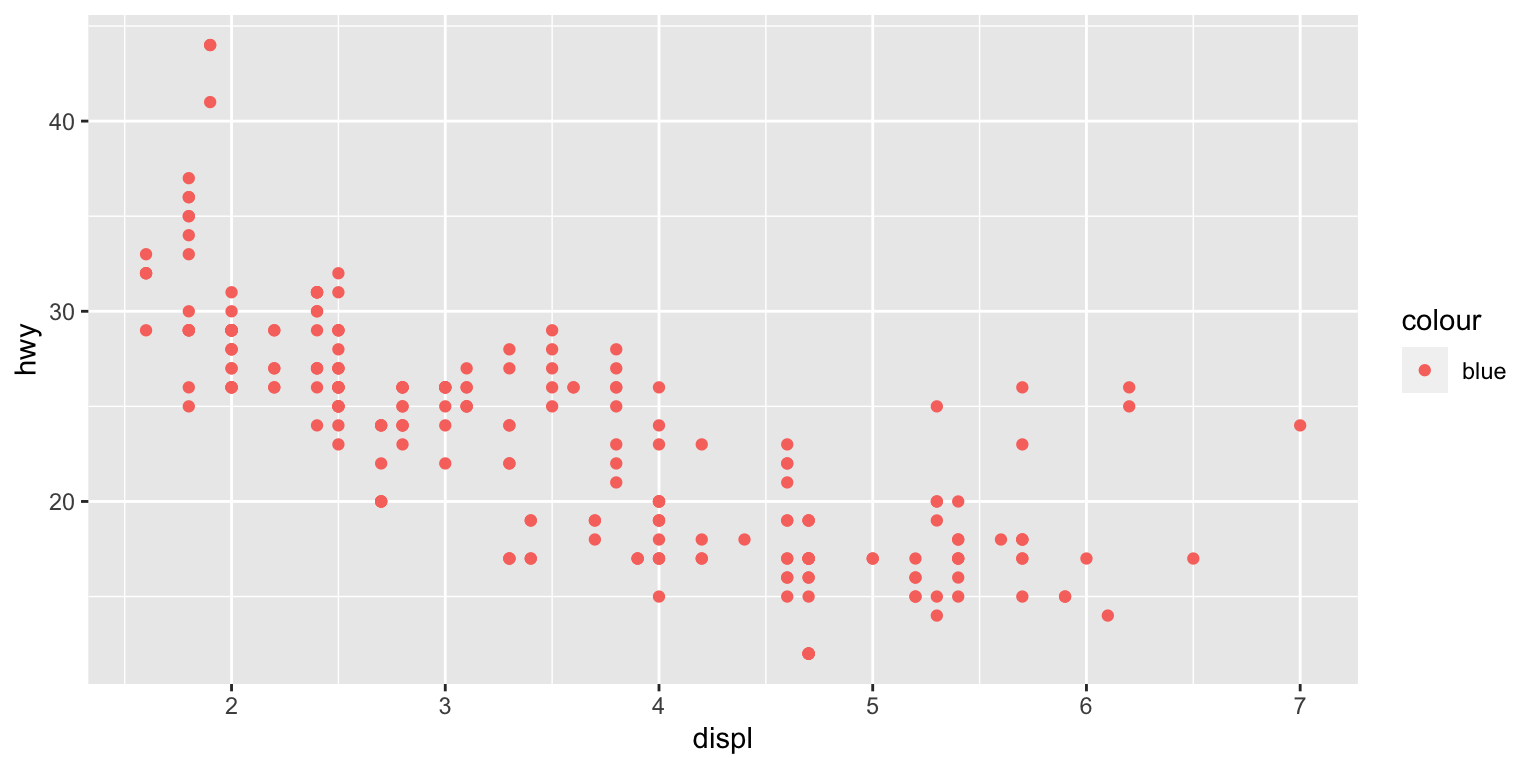
\includegraphics{week2_files/figure-latex/unnamed-chunk-8-1} \end{center}

\begin{Shaded}
\begin{Highlighting}[]
\KeywordTok{ggplot}\NormalTok{(dataset, }\KeywordTok{aes}\NormalTok{(displ, hwy)) }\OperatorTok{+}\StringTok{ }\KeywordTok{geom_point}\NormalTok{(}\DataTypeTok{colour =} \StringTok{"blue"}\NormalTok{)}
\end{Highlighting}
\end{Shaded}

\begin{center}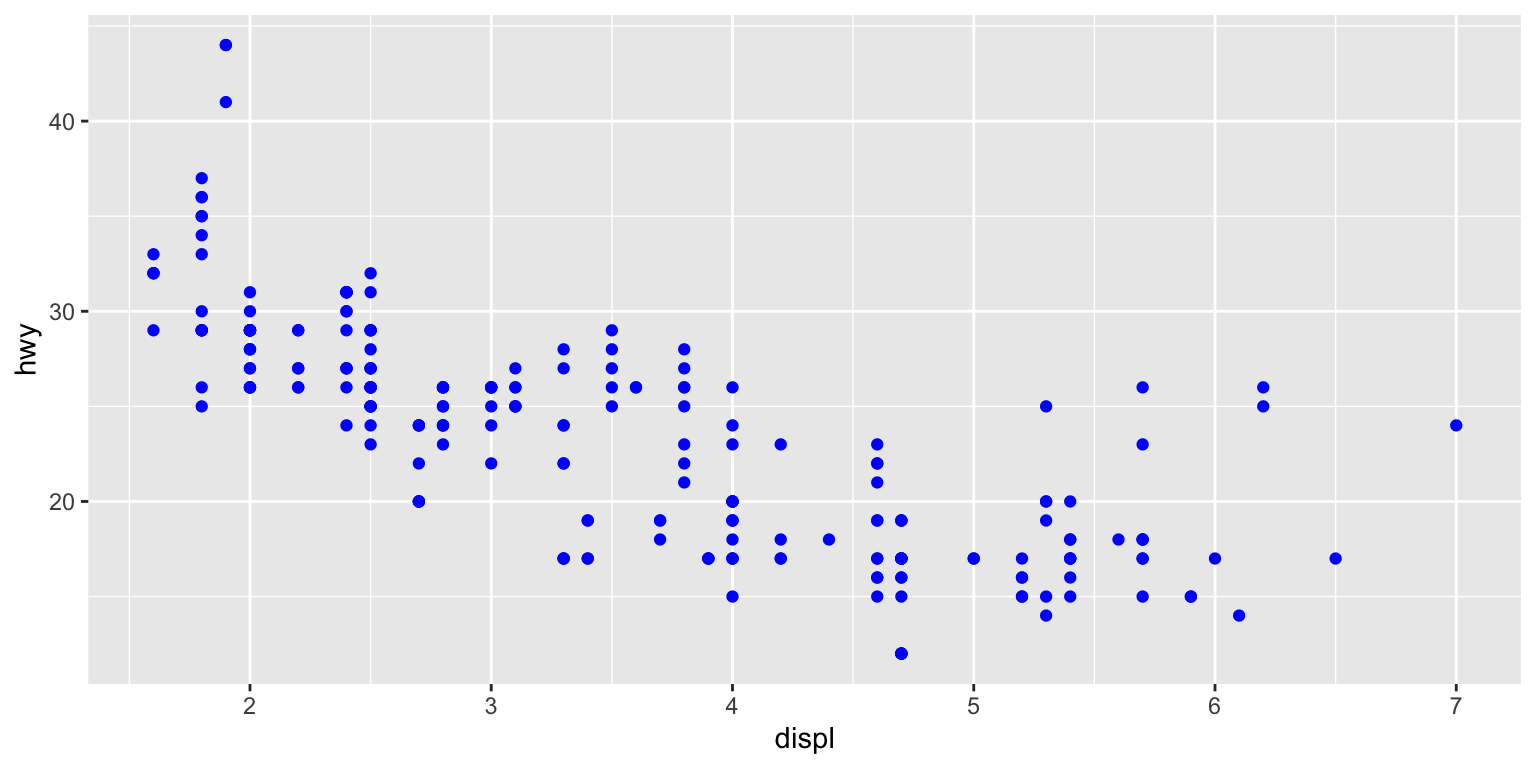
\includegraphics{week2_files/figure-latex/unnamed-chunk-8-2} \end{center}

\textbf{Important} - Colour and shape work well with categorical
variables - Size works well for continuous variables. - if there is a
lot of data it can be hard to distinguish different groups. - For the
multiple groups use facetting

\textbf{Tasks}

\begin{itemize}
\item
  Experiment with the colour, shape and size aesthetics. What happens
  when you map them to continuous values? What about categorical values?
  What happens when you use more than one aesthetic in a plot?
\item
  What happens if you map a continuous variable to shape? Why? What
  happens if you map trans to shape? Why?
\item
  How is drive train related to fuel economy? How is drive train related
  to engine size and class?
\end{itemize}

\hypertarget{facetting}{%
\paragraph{Facetting}\label{facetting}}

\textbf{Facetting} creates tables of graphics by splitting the data into
subsets and displaying the same graph for each subset.

There are two types of facetting: - grid - wrapped - most useful

\end{document}
